% Created 2018-11-16 Fri 08:36
% Intended LaTeX compiler: pdflatex
\documentclass[presentation]{beamer}
\usepackage[utf8]{inputenc}
\usepackage[T1]{fontenc}
\usepackage{graphicx}
\usepackage{grffile}
\usepackage{longtable}
\usepackage{wrapfig}
\usepackage{rotating}
\usepackage[normalem]{ulem}
\usepackage{amsmath}
\usepackage{textcomp}
\usepackage{amssymb}
\usepackage{capt-of}
\usepackage{natbib}
\usepackage[linktocpage,pdfstartview=FitH,colorlinks,
linkcolor=blue,anchorcolor=blue,
citecolor=blue,filecolor=blue,menucolor=blue,urlcolor=blue]{hyperref}
\setbeamertemplate{frame footer}{\insertshortauthor}
\setbeamerfont{page number in head/foot}{size=\tiny}
\setbeamercolor{footline}{fg=gray}
\usepackage{amsmath}
\author{Florian Hollenbach}
\usepackage[english]{isodate}
\usepackage{amsmath,amsthm,amssymb,amsfonts}
\newcommand{\E}{\mathbb{E}}
\newcommand{\V}{\mathbb{V}}
\usetheme{metropolis}
\usecolortheme{}
\usefonttheme{}
\useinnertheme{}
\useoutertheme{}
\author{Florian Hollenbach}
\date{\today}
\title{Political Science 209 - Fall 2018}
\subtitle{Uncertainty}

\hypersetup{
 pdfauthor={Florian Hollenbach},
 pdftitle={Political Science 209 - Fall 2018},
 pdfkeywords={},
 pdfsubject={},
 pdfcreator={Emacs 25.3.1 (Org mode 9.1.14)}, 
 pdflang={English}}
\begin{document}

\maketitle


\begin{frame}[label={sec:org6e32cd4}]{Statistical Inference}
Goal: trying to estimate something unobservable from observable data

What we want to estimate: \alert{parameter} \(\theta\) \(\rightsquigarrow\) unobservable

What you do observe: \alert{data}

\pause

We use data to compute an estimate of the parameter \(\hat\theta\)
\end{frame}


\begin{frame}[label={sec:org5690295}]{Parameters and Estimators}
\begin{itemize}
\item \alert{parameter}: the quantity that we are interested in
\end{itemize}

\pause

\begin{itemize}
\item \alert{estimator}: method to compute parameter of interest
\end{itemize}
\end{frame}

\begin{frame}[label={sec:org7b22cae}]{Parameters and Estimators}
Example:

\begin{itemize}
\item \alert{parameter}: support for Jimbo Fisher in student population

\item \alert{estimator}: sample proportion of support as estimator
\end{itemize}
\end{frame}

\begin{frame}[label={sec:org68b16f4}]{Parameters and Estimators}
Example:

\begin{itemize}
\item \alert{parameter}: average causal effect of aspirin on headache

\item \alert{estimator}: difference in mean between treatment and control
\end{itemize}
\end{frame}


\begin{frame}[label={sec:org25a667b}]{Quality of estimators}
For the rest of the semester the question becomes:

\alert{How good is our estimator?}

\pause

\begin{enumerate}
\item \alert{How close in expectation is the estimator to the truth?}

\item \alert{How certain or uncertain are we about the estimate?}
\end{enumerate}
\end{frame}

\begin{frame}[label={sec:org94ea43c}]{Quality of estimators}
How good is \(\hat\theta\) as an estimate of \(\theta\)?

\begin{itemize}
\item Ideally, we want to know \alert{estimation error} \(= \hat\theta - \theta_{truth}\)
\end{itemize}

But we can never calculate this. Why?

\pause

\(\theta_{truth}\) is unknown

\emph{If we knew what the truth was, we didn't need an estimate}
\end{frame}

\begin{frame}[label={sec:org789aa63}]{Quality of estimators}
Instead, we consider two hypothetical scenarios:
\begin{enumerate}
\item How well would \(\hat\theta\) perform over \emph{repeated data generating processes}? (\alert{bias})
\item How well would \(\hat\theta\) perform as the sample size goes to infinity? (\alert{consistency})
\end{enumerate}
\end{frame}

\begin{frame}[label={sec:orge023b95}]{Bias}
\begin{itemize}
\item Imagine the estimate being a random variable itself

\item Drawing infinitely many samples of students asking about Jimbo
\end{itemize}

What is the average of the sample average? Or what is the expectation of the estimator?

bias = \(\E\)(estimation error) = \(\E\)(estimate - truth) = \(\E(\bar{X})\) - p = p - p = 0
\end{frame}


\begin{frame}[label={sec:org19996e9}]{Bias - \alert{Important}}
\alert{An unbiased estimator does not mean that it is always exactly correct!}

\pause
\alert{To remember:} bias measures whether in expectation (on average) the estimator is giving us the truth
\end{frame}

\begin{frame}[label={sec:orge90b0e5}]{Consistency}
Essentially saying that the law of large numbers applies to the estimator, i.e.:

\alert{An estimator is said to be consistent if it converges to the parameter (truth) if N goes to \(\infty\)}
\end{frame}


\begin{frame}[label={sec:orgcecaa84}]{Variability}
Next, we have to consider how certain we are about our results

Consider two estimators:

\begin{enumerate}
\item slightly \emph{biased}, on average off by a bit, but always by the same margin

\item unbiased, but misses target left and right
\end{enumerate}
\end{frame}


\begin{frame}[label={sec:org09e5657}]{Variability}
\begin{center}
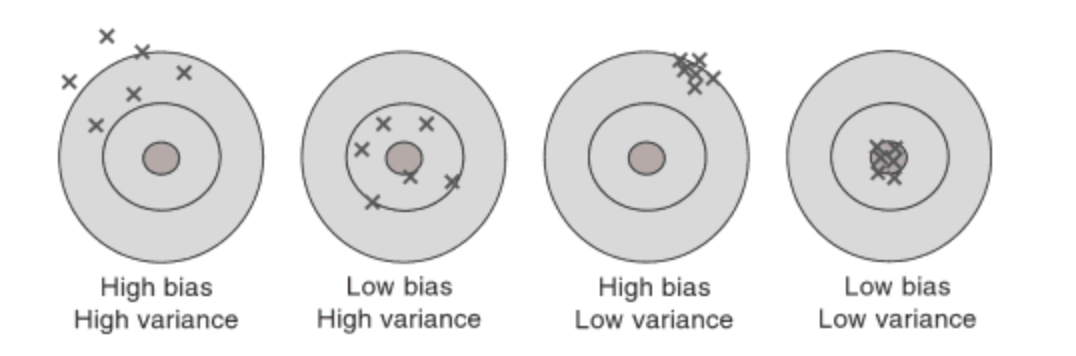
\includegraphics[width=6cm]{/Users/florianhollenbach/Documents/GitHub/Polisci209_2018/slides/week13/DART.png}
\end{center}

(Encyclopedia of Machine Learning)
\end{frame}

\begin{frame}[label={sec:orga418a98}]{Variability}
We characterize the variability of an estimator by using the standard deviation of the sampling distribution

\alert{How do we find that????}

\pause

Remember, the sampling distribution is the distribution of our statistic over hypothetical infinitely many samples
\end{frame}

\begin{frame}[label={sec:org2079ffd}]{Variability}
\begin{center}
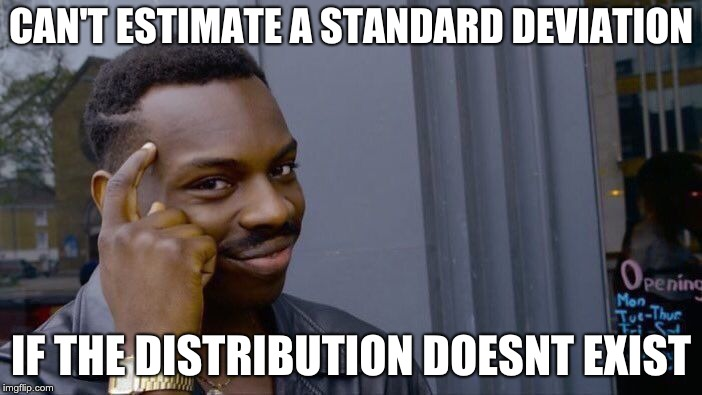
\includegraphics[width=6cm]{/Users/florianhollenbach/Documents/GitHub/Polisci209_2018/slides/week13/2mi1j5.jpg}
\end{center}
\end{frame}


\begin{frame}[label={sec:org4226bdd}]{Standard Error}
We estimate the standard deviation of the sampling distribution from the observed data

\alert{standard error}

\pause

``\emph{standard error} and describes the (estimated) average degree to which an estimator deviates from its expected value'' (Imai 2017)
\end{frame}

\begin{frame}[label={sec:org88e4602}]{Polling Example}
Say we took a sample of 1000 students and asked whether they support Jimbo or not

Define a random variable \(X_{i} = 1\) if student \emph{i} supports Jimbo, \(X_{i}=0\) if not

Binomial distribution with success probability p and size N where p is the proportion of \emph{all students} who support Jimbo (population dist)
\end{frame}


\begin{frame}[label={sec:org7ae15ce}]{Polling Example}
Estimator: ?
\end{frame}

\begin{frame}[label={sec:orgbfcc568}]{Polling Example}
Estimator: \(\overline{X} = \frac{1}{N} \sum_{i=1}^{N} X_{i}\)

\pause

In earlier notation: \(\theta_{truth} =p\) and \(\theta = \overline{X}\)
\end{frame}


\begin{frame}[label={sec:org11a177f}]{Polling Example}
Estimator: \(\overline{X} = \frac{1}{N} \sum_{i=1}^{N} X_{i}\)

\begin{enumerate}
\item LLN: \(\overline{X} \longrightarrow p\) (\alert{consistent})

\item Expectation: \(\E(\overline{X}) = p\) (\alert{unbiased})

\item standard error?
\end{enumerate}
\end{frame}


\begin{frame}[label={sec:org2d35040}]{Polling Example - standard error}
\(X_i\) are i.i.d Bernoulli random variables with probability = p


\(\V(\overline{X}) = \frac{1}{N^{2}} \V(\sum_{i=1}^{N}X_{i})  = \frac{1}{N^{2}} \sum_{i=1}^{N} \V(X_{i})\)
\end{frame}


\begin{frame}[label={sec:org7c2d71d}]{Polling Example - standard error}
\(X_i\) are i.i.d Bernoulli random variables with probability = p


\(\V(\overline{X}) = \frac{1}{N^{2}} \V(\sum_{i=1}^{N}X_{i})  = \frac{1}{N^{2}} \sum_{i=1}^{N} \V(X_{i}) = \frac{N}{N^{2}} \V(X)\)
\end{frame}


\begin{frame}[label={sec:orgceef2d3}]{Polling Example - standard error}
\(X_i\) are i.i.d Bernoulli random variables with probability = p


\(\V(\overline{X}) = \frac{1}{N^{2}} \V(\sum_{i=1}^{N}X_{i})  = \frac{1}{N^{2}} \sum_{i=1}^{N} \V(X_{i}) = \frac{N}{N^{2}} \V(X) = \frac{p \times (1-p)}{N}\)
\end{frame}

\begin{frame}[label={sec:orgafeb639}]{Polling Example - standard error}
\(\V(\overline{X}) = \frac{p \times (1-p)}{N}\)

Standard error: \(\sqrt{\V(\overline{X})}\)

But we don't know p! Now what?

\pause

We use our unbiased estimate of p: \overline{X}
\end{frame}

\begin{frame}[label={sec:org723924c}]{Polling Example - standard error estimate}
\(\sqrt{\widehat{\V(\overline{X})}} = \sqrt{\frac{\overline{X}(1-\overline{X})}{N}}\)
\end{frame}

\begin{frame}[label={sec:org06e6230}]{Polling Example - standard error estimate}
Assume in our sample 55\% of students support Jimbo:

SE = \(\sqrt{\widehat{\V(\overline{X})}} = \sqrt{\frac{0.55 \times (1-0.55)}{1500}} = \sqrt{\frac{0.55 \times (0.45)}{1500}} = 0.013\)

We can expect our estimate on average to be off by 1.3 percentage points

\pause

If \(\overline{X}\) = 0.8, then SE = 0.010

If N = 500, \(\overline{X}\) = 0.55, then SE = 0.022
\end{frame}

\begin{frame}[label={sec:org5ac2971}]{Standard error estimate}
Standard error is based on variance of the sampling distribution

Gives estimate of uncertainty

Each estimator/statistic has unique sampling distribution, e.g. difference in means
\end{frame}

\begin{frame}[label={sec:org2bf089a}]{Confidence Intervals}
Often we don't even know the sampling distribution of our estimators

How could we approximate it?


\pause
\alert{Central limit theorem!}
\end{frame}


\begin{frame}[label={sec:org8df1c8d}]{Confidence Intervals}
Central limit theorem says:

\(\overline{X} \approx N(\E(X), \frac{\V(X)}{N})\)

\alert{regardless of distribution of X}
\end{frame}


\begin{frame}[label={sec:org836f54e}]{Confidence Intervals}
We can use the approximation to the sampling distribution, \(\overline{X} \approx N(\E(X), \frac{\V(X)}{N})\) to construct \alert{confidence intervals}

Confidence intervals give a range of values that is likely to contain the true value

\pause
To start, we select a probability value for our confidence level: usually 95$\backslash$%
\end{frame}

\begin{frame}[label={sec:org7c01b19}]{Confidence Intervals}
\alert{The 95\% confidence interval specifies the range of values in which the true parameter will fall for 95\% of our hypothetical samples/experiments}

\pause

Put differently
\alert{``Over a hypothetically repeated data generating process, confidence intervals contain the true value of parameter with the probability specified by the confidence level''} (Imai 2017)
\end{frame}


\begin{frame}[label={sec:orgb13044c}]{Confidence interval}
(1-\(\alpha\)) large sample Confidence interval is defined as:

CI(\(\alpha\)) = \(\overline{X} - z_{\frac{\alpha}{2}} \times SE\),  \(\overline{X} + z_{\frac{\alpha}{2}} \times SE\)

\(z_{\frac{\alpha}{2}}\) is the critical value which equals \((1 − \frac{\alpha}{2})\) quantile of the standard normal distribution
\end{frame}

\begin{frame}[label={sec:org392c215}]{Confidence interval}
Where do the critical values come from?

\pause
Remember: Curve of the standard normal distribution:

\begin{itemize}
\item Symmetric around 0
\item Total area under the curve is 100\%
\item Area between -1 and 1 is \textasciitilde{}68\%
\item Area between -2 and 2 is \textasciitilde{}95\%
\item Area between -3 and 3 is \textasciitilde{}99.7\%
\end{itemize}
\end{frame}

\begin{frame}[label={sec:org3ae94a8}]{Confidence interval}
\begin{center}
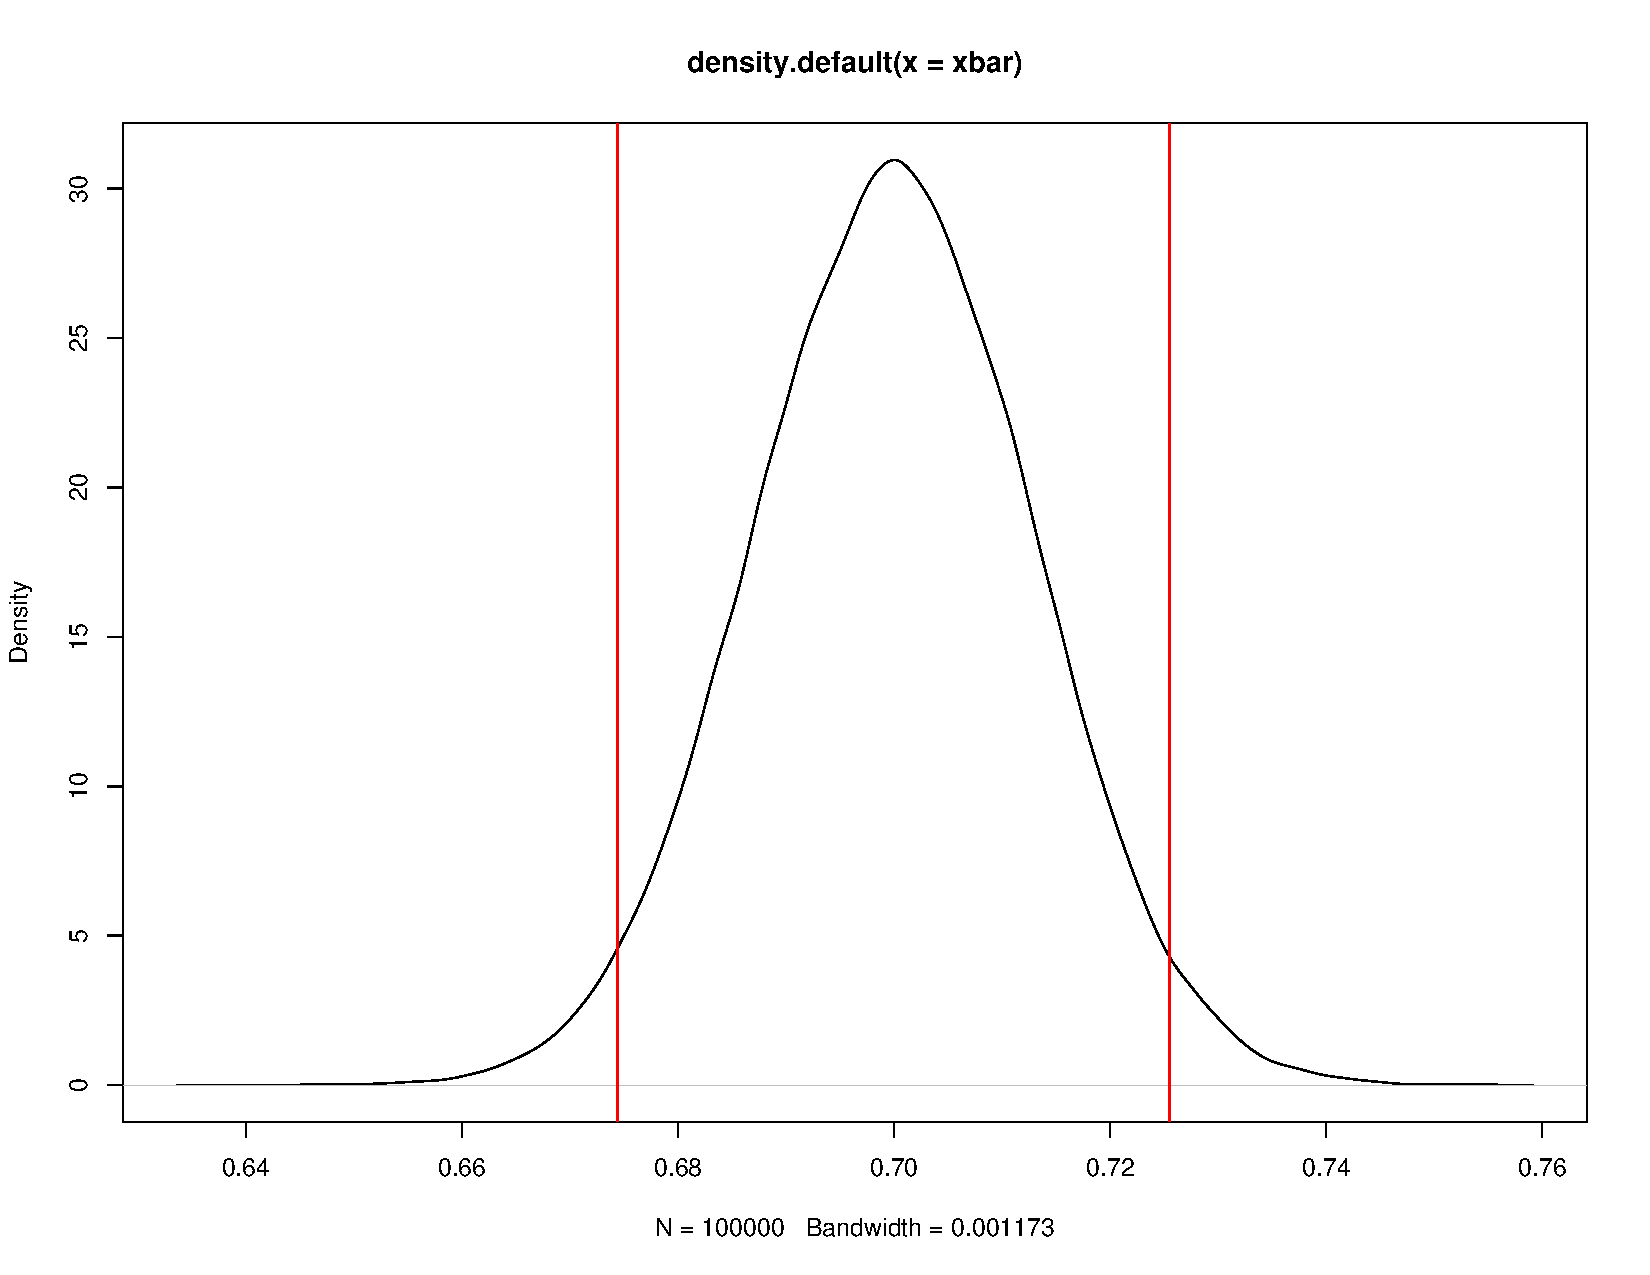
\includegraphics[width=6cm]{/Users/florianhollenbach/Documents/GitHub/Polisci209_2018/slides/week13/Norm_density.pdf}
\end{center}

\alert{Critical values are the exact vales between which the standard normal distribution will include (1-\(\alpha\)) \% of the area}
\end{frame}

\begin{frame}[label={sec:org2c50225}]{Confidence interval interpretation}
Technically the CI is \alert{not} the probability of the true parameter being between the two value.

\pause
Remember, in our view the true parameter is fixed

Instead: ``955\% confidence intervals contain the true value of the parameter 95\% of the time during a hypothetically repeated data generating process'' (Imai 2017)
\end{frame}

\begin{frame}[label={sec:org8e55df3}]{Confidence interval interpretation}
Remember in the Jimbo example with \(\overline{X} = 0.55\) and N = 1500

SE = \(\sqrt{\widehat{\V(\overline{X})}} = \sqrt{\frac{0.55 \times (1-0.55)}{1500}} = \sqrt{\frac{0.55 \times (0.45)}{1500}} = 0.013\)
\end{frame}

\begin{frame}[label={sec:orgd7cb02d}]{Confidence interval}
CI(\(\alpha\)) = \(\overline{X} - z_{\frac{\alpha}{2}} \times SE\),  \(\overline{X} + z_{\frac{\alpha}{2}} \times SE\)

\pause

CI(0.05) = \(0.55 - 1.96 \times 0.013\),  0.55 +  1.96 \texttimes{} 0.013\$ = 0.524, 0.576
\end{frame}


\begin{frame}[fragile,label={sec:orga651d90}]{Confidence interval}
 What if we don't know the variance of the estimator?

Let's use the variance of the sample?

\begin{verbatim}
x <- rbinom(1000,1,0.7)
var <-var(x)/1500
SE <- sqrt(var)
\end{verbatim}

SE = 0.013
\end{frame}


\begin{frame}[fragile,label={sec:orga2016c8}]{Confidence interval}
 \begin{verbatim}
xbar <- rep(NA, 10000)
for(i in 1:10000){
  x <- rbinom(1000,1,0.7)
  xbar[i] <-mean(x)
}
\end{verbatim}

Write an R-script to test our confidence interval for Jimbo!
\end{frame}
\end{document}